\documentclass[11pt]{article}
\usepackage[utf8]{inputenc}
%\usepackage[T1]{fontenc}
\usepackage{amssymb}
\usepackage{amsmath}
\usepackage{enumerate}
\usepackage{fullpage}
\usepackage{polski}  
\usepackage{indentfirst} 
\usepackage[pdftex]{graphicx}
\usepackage{multirow}
\usepackage{placeins}

\author{Łukasz Dubiel}
\title{Matematyka \\Liczby zespolone}
\date{15 grudnia 2011 \\ 20 grudnia 2011 \\ 3 stycznia 2012}
\begin{document}

\maketitle

$$W(x) = a_n x^n + \ldots + a_1x + a_0 \quad a_1 \in \mathbb{R} \quad \forall i$$

$$ \mathbb{N} \subset \mathbb{Z} \subset \mathbb{Q} \subset \mathbb{R} \subset \mathbb{C}$$

\section{Definicja $i$ oraz $\mathbb{C}$}
$i$ definiujemy jako rozwiązanie równania
$$x^2 + 1 = 0$$
Wtedy dostajemy $\mathbb{C}$ to
$$ \mathbb{C} := \left\lbrace a + ib \quad a,b \in \mathbb{R}, \ i^2 = -1 \right\rbrace$$
\subsection{Definicja - postać algebraiczna}
$$ z = x + iy$$
$$ x = \Re{z} $$
$$ y = \Im{z} $$
\subsection{Stwierdzenie o równości liczb zespolonych}
$$ z_1 = z_2 \iff \Re{z_1} = \Re{z_2} \wedge \Im{z_1} = \Im{z_1}$$
\section{Działania na liczbach zespolonych w postaci algebraicznej}
$z_1, z_2 \in \mathbb{C}$ \\
$z_1 = x_1 + iy_2$ \\
$z_2 = x_2 + iy_2$
\subsection{Dodawanie}
$$z_1 + z_2 = (x_1 + iy_1) + (x_2 + iy_2) = (x_1 + x_2) + i(y_1 + y_2)$$
$$\Re(z_1 + z_2) = \Re(z_1) + \Re(z_2)$$
$$\Im(z_1 + z_2) = \Im(z_1) + \Im(z_2)$$
\subsection{Odejmowanie}
$$z_1 - z_2 = (x_1 - iy_1) - (x_2 - iy_2) = (x_1 - x_2) - i(y_1 - y_2)$$
$$\Re(z_1 - z_2) = \Re(z_1) - \Re(z_2)$$
$$\Im(z_1 - z_2) = \Im(z_1) - \Im(z_2)$$
\subsection{Mnożenie}
$$z_1 z_2 = (x_1 + iy_2)(x_2 + iy_2) = (x_1x_2 - y_1y_2) + i(x_1y_2 + y_1x_2)$$
\subsection{Dzielenie}
$$\frac{z_1}{z_2} = \frac{x_1 +iy_1}{x_2 + iy_2} = \frac{(x_1 + iy_1)(x_2 - iy_2)}{(x_2 +iy_2)(x_2 - iy_2)} = \frac{(x_1x_2 + y_1y_2) + i(y_1x_2 - x_1y_2)}{x_2^2 +y^2} $$
\section{Twierdzenie - własności działań w zobierze liczb zespolonych}
\subsection{Łączność}
$$ \forall z_1,z_2,z_3 \in \mathbb{C} \quad (z_1 + z_2) + z_3 = z_1 + (z_2 + z_3)\\
(z_1z_2)z_3 = z_1(z_2z_3)$$
\subsection{Przemienność}
$$\forall z_1,z_2 \in \mathbb{C} \quad z_1 + z_2 = z_2 + z_1 \\
z_1z_2 = z_2z_2$$
\subsection{Rozdzielność mnożenia względem dodawania}
$$\forall z_1,z_2,z_3 \in \mathbb{C} \quad (z_1 + z_2) z_3 = (z_1z_3 + z_2z_3)$$

\section{Interpretacja geometryczna}
$$x + iy = z ~ (x,y) , \quad x,y \in \mathbb{R}$$
\begin{center}
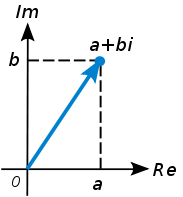
\includegraphics[scale=0.6]{interpretacja.png}
\end{center}
\section{Sprzężenie}
Zprzeżeniem liczby $z = x + iy $ nazywamy liczbę:
$$\overline{z} = x - iy$$
\begin{center}
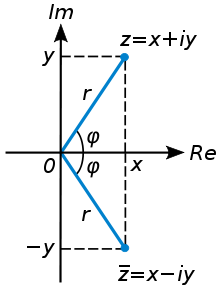
\includegraphics[scale=0.6]{sprzezenie.png}
\end{center}

\subsection{Uwaga o sprzężeniu}
$z \in \mathbb{C}$
$$ z = \overline{z} \iff z \in \mathbb{R}$$

\section{Moduł}
Modułem liczby zespolonej $z = x + iy $ nazywamy liczbę
$$ |z| = \sqrt{x^2 + y^2} $$

\subsection{Uwaga o kole i innych kołowych figurach}
Koło możemy również zdefiniować jako
$$ \{ z \in \mathbb{C} : |z| \leq r , r \in \mathbb{R} \}$$

Wyrażenie $ |z_1 - z_2| $ jest odległością dzielącą dwa punkty na płaszczyźnie zespolonej, tak więc możemy zdefiniować koło w punkcie różnym od $(0,0)$
$$ \{ z \in \mathbb{C} : | z - z_0| < r , r \in \mathbb{R}, z_0 \in \mathbb{C}\}$$

Kolejna ciekawa figura

$z_0 \in \mathbb{C}, \quad r,R \in \mathbb{R}$ 
$$\{ z \in \mathbb{C} : r < | z - z_0 | < R \}$$
Takie coś nazywamy pierścieniem kołowym

\subsection{Twierdzenia}
$z_1, z_2 \in \mathbb{C}$
$$\overline{z_1} \cdot \overline{z_2}  = \overline{z_1\cdot z_2}$$
$z_2 \not = 0$
$$ \frac{\overline{z_1}}{\overline{z_2}} = \overline{\left(\frac{z_1}{z_2}\right)}$$
$$ \overline{z_1} + \overline{z_2} = \overline{z_1 + z_2}$$
$$ \overline{\overline{z}} = z$$

$$ |z_1| \cdot |z_2| = |z_1 \cdot z_2| $$
$z_2 \not = 0$
$$ \frac{|z_1|}{|z_2|} = \left|\frac{z_1}{z_2}\right|$$

$$ |z_1 + z_2| \leq |z_1| + |z_2|$$

\newpage
\section{Postać trygonometryczna}
\begin{center}
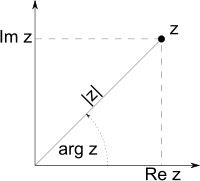
\includegraphics[scale=0.6]{trygonometrzyczna.png}
\end{center}

Dostajemy
$$\begin{cases}
\cos{\varphi} = \frac{\Re{z}}{|z|} \\
\sin{\varphi} = \frac{\Im{z}}{|z|} 
\end{cases}$$

$$ z = \Re{z} + i \Im{z} = |z|\cos{\varphi} + i|z|\sin{\varphi} = |z|(\cos{\varphi} + i \sin{\varphi})$$
Zapis :
$$ z = |z|(\cos{\varphi} + i \sin{\varphi})$$
nazywamy zapisem trygonometryczna liczby zespolonej.
\subsection{Definicja}
Argumentem liczby zespolonej $z = x + iy \not = 0 \quad x,y \in \mathbb{R}$ nazywamy liczbę $ \varphi \in \mathbb{R}$ spełniającą układ równań 
$$\begin{cases}
\cos{\varphi} = \frac{\Re{z}}{|z|} \\
\sin{\varphi} = \frac{\Im{z}}{|z|} 
\end{cases}$$
Zbiór $\varphi$ spełniających ten układ równań oznacza się
$$ \arg{z} $$
przyjmuje się że $\arg 0 = \mathbb{R}$
\subsection{Wniosek}
$z \not = 0$
Dla $\varphi_1,\varphi_2 \in \arg{z}$ można zapisać
$$ \varphi_1 = \varphi_2 + 2k\pi \quad k \in \mathbb{Z}$$

\subsection{Definicja argumentu głównego}
Argumentem główny liczby zespolonej $z \not = 0 $ nazywamy tę pośród $\arg z$ która należy do przedziału $<0,2\pi)$
\subsection{Stwierdzenie}
$z \not = 0$
$$ \arg{\overline{z}} = 2\pi - \arg{z}$$
oraz przyjmujemy że $\arg{0} = 0 $ ( argument główny )
\subsection{Przykład}
$$ \{ z \in \mathbb{C} : \arg z = 0\} $$
I dostajemy $\mathbb{R}_+ \cup {0}$

\subsection{Równość liczb w postaci trygonometrycznej}
$ z_1,z_2 \in \mathbb{C}$ \\
$ z_1 = |z_1|(\cos{\varphi_1} + i\sin{\varphi_1}),\ \varphi_1 \in \arg z_1$\\
$ z_2 = |z_2|(\cos{\varphi_2} + i\sin{\varphi_2}) \varphi_2 \in \arg z_2$\\

$$ z_1 = z_1 \iff \begin{cases} |z_1| = |z_2| \wedge \varphi_1 = \varphi_2 + 2k\pi, \quad |z_1| \not = 0, |z_2| \not = 0, k \in \mathbb{Z}\\ |z_1| = |z_2|\quad |z_1| = |z_2| = 0 \end{cases}$$

\subsection{Mnożenie}
$ z_1,z_2 \in \mathbb{C}$ \\
$ z_1 = |z_1|(\cos{\varphi_1} + i\sin{\varphi_1}),\ \varphi_1 \in \arg z_1$\\
$ z_2 = |z_2|(\cos{\varphi_2} + i\sin{\varphi_2}),\ \varphi_2 \in \arg z_2$\\
$$ z_1 \cdot z_2 = |z_1| \cdot |z_2|\left[ ( \cos{\varphi_1}\cos{\varphi_2} - \sin{\varphi_1}\sin{\varphi_2}) + i(\cos{\varphi_1}\sin{\varphi_2} + \sin{\varphi_1}\cos{\varphi_2})\right]$$
$$ z_1 \cdot z_2 = |z_1| \cdot |z_2|( \cos{(\varphi_1 + \varphi_2)} + i \sin{(\varphi_1 + \varphi_2)})$$

\subsection{Wniosek o dzieleniu}
$z_2 \not = 0$
$$\frac{z_1}{z_2} = \frac{|z_1|}{|z_2|}(\cos{(\varphi_1 - \varphi_2)} + i\sin{(\varphi_1 - \varphi_2)})$$
\subsection{Wniosek o potęgowaniu}
$ z \in \mathbb{C}$ \\
$ z = |z|(\cos{\varphi} + i\sin{\varphi}),\ \varphi \in \arg z_1$\\
$n \in \mathbb{N}$

Wtedy
$$ z^n = |z|^n ( \cos{n\varphi} + i\sin{n\varphi}) $$
te wzroki to wzory de Moivre'a

\subsection{Przykład}
$$ (1 + i ) ^{100}  = ( \sqrt{2} ( \cos{\frac{\pi}{2}} + i \sin{\frac{\pi}{4}})^{100} = 2^{50} ( \cos{\frac{100\pi}{4}} + i\cos{\frac{100\pi}{4}}) = 2^{50} ( \cos{\pi} + i \sin{\pi} ) = -2^{50}$$
\subsection{Stwierdzenie}
$$z_1,z_2 \in \mathbb{C}$$
$$\arg(z_1 \cdot z_2 ) = \arg{z_1} + \arg{z_2} + 2k_1\pi $$
Ale to $k_1$ ma być w $\mathbb{Z}$ ale je wyznaczyć explicite
$$ k_1 = \lfloor \frac{z_1 + z_2}{2\pi} \rfloor \pi$$
Analogicznie
$$ \arg{\frac{z_1}{z_2}} = \arg{z_1} - \arg{z_2} + 2k_2 \pi $$
Podobnie jak w poprzednim $k_2$ ma być w $\mathbb{Z}$ ale można ją wyznaczyć explicite.
$$ k_1 = \lfloor \frac{z_1 - z_2}{2\pi} \rfloor \pi$$
Podczas potęgowania
$$ \arg{z_1^n} = n \arg{z_1} + 2k_3\pi $$
Podobnie $k_3 \in \mathbb{Z}$ ale też można wyznaczyć explicite.

\section{Zapis wykładniczy}
\subsection{Wzór Eulera}
$$ e^{i\varphi} = \cos{\varphi} + i\sin{\varphi} $$
\subsection{Definicja}
$$ z = |z|e^{i\varphi} $$
\section{Najpiękniejszy wzór matematyki}
$$ e^{i\varphi} + 1 = 0 $$
\section{Pierwiastkowanie}
$ n \in \mathbb{N}^+ $ $$ w^n = z \Longrightarrow w = \sqrt[n]{z} $$

$$ z = |z| ( \cos{\varphi} + i \sin{\varphi} ) , \quad \varphi \in \arg{z} $$
$$ w = |w| ( \cos{\psi} + i \sin{\psi} ), \quad \psi \in \arg{z}$$
Korzystając z wzoru de'Movara zapisujemy obie liczb
$$ |w|^n(\cos{n\psi} + i\sin{n\psi} ) = |z| ( \cos{\varphi} + i\sin{\varphi}) $$
Korzystając z warunków równości możemy zapisać
$$ \begin{cases} |w|^n = |z| \\ n\psi = \varphi + 2k\pi\end{cases}$$
Zajmijmy się równaniem drugim
$$ \begin{cases} |w| = \sqrt[n]{|z|} \\ \psi = \frac{\varphi + 2k\pi}{n} \end{cases}$$
I teraz zauważamy, że dla ka całkowitego zbór $\psi$ jest skończony ( jest pierścieniem cyklicznym )
$$ w = \sqrt[n]{|z|}\left(\cos{\frac{\varphi + 2k\pi}{n}} + i \sin{\frac{\varphi +2k\pi}{n}}\right), \quad k \in \{0 \ldots n-1\}$$
Czyli jeśli $z \not = 0$
$$ \sqrt[n]{z} = \{z_0,\ldots,z_{n-1}\} $$ gdzie
$$ z_k = \sqrt[n]{|z|}\left(\cos{\frac{\varphi + 2k\pi}{n}} + i \sin{\frac{\varphi +2k\pi}{n}}\right), \quad k \in \{0 \ldots n-1\}$$
\subsection{Uwaga}
Jeśli
$$ z_0 = \sqrt[n]{|z|}\left(\cos{\frac{\arg{z}}{n}} + i \sin{\frac{\arg{z}}{n}}\right)$$
to
$$ z_{k+1} = z_k(\cos{\frac{2\pi}{n}} + i \cos{\frac{2\pi}{n}})= 
z_0\left(\cos{\frac{2\pi}{n}} + i\sin{\frac{2\pi}{n}}\right)^{k+1}$$

Zbór punktów tworzony przez pierwiastek $n$-tego stopnia  z liczby zespolonej $z$ jest $n$-kątem foremny wpisanym do koła o promieniu $\sqrt{z}$.
\newpage
\subsection{Przykład}
$ \sqrt[4]{1} $
oraz
$ \sqrt{1} $

\subsection{Przykład}
$ \sqrt[3]{8} $
$$ 8 = 9 ( \cos{0} + i\sin{0} )$$
$$ w_0 = 2 (\cos{0} + i\sin{0} ) = 2$$
$$ w_1 = 2 (\cos{\frac{2\pi}{3}} + i\sin{\frac{2\pi}{3}}) = 2(-\frac{1}{2} + i\frac{\sqrt{3}}{2}$$
$$ w_2 = 2 (\cos{\frac{4\pi}{3}} + i\sin{\frac{4\pi}{3}}) = 2(-\frac{1}{2} + i\frac{-\sqrt{3}}{2})$$
\subsection{Przykład 2}
$$\sqrt[4]{(2+2i)^8}$$
$$ w^4 = (2+2i)^8 = \left[(2+2i)^2\right]^4 $$
$$(2+2i)^2 = \left[2\sqrt{2}\left(\cos{\frac{\pi}{4}} + i \sin{\frac{\pi}{2}}\right)\right] =  8i $$
Interpretacja geometryczna
$$ \sqrt[4]{(2+2i)^8} = \{ 8i , -8, -8i , 8 \} $$

\section{Zasadnicze twierdzenie algebry - twierdzenie gaussa}
Dowolny wielomian stopnia $n$ o współczynnikach zespolonych ( w szczególności rzeczywistych ) ma dokładnie $n$ pierwiastków zespolonych licząc z krotnościami.

\subsection{Uwaga}
Mówimy, że zbór liczb zespolonych jest algebraicznie domknięty. 

\newpage
\subsection{Twierdzenie}
Niech
$$ W(x) = \sum_{i=1}^{n} a_ix^i , \quad n \not = 0 , \quad a_i \in \mathbb{R} \quad  \forall\ i \leq n $$
$$ W(z_0) = 0 \Longrightarrow W(\overline{z_0}) = 0$$
$$ W(z_0) = \sum_{i=1}^{n} a_iz_0^i = 0$$
$$\overline{\sum_{i=1}^{n} a_ix^i} = \sum_{i=1}^{n} \overline{a_i z_0^i} = \overline{0}$$
$$ \sum_{i=1}^{n} a_i\overline{z_0}^i = W(\overline{z_0}) $$

\section{Twierdzenie}
Jeżeli mamy wielomian o nieparzystym stopniu to istnieje przynajmniej pierwiastek rzeczywisty
\subsection{Dowód}
Natychmistowy z własności Darboux.

\subsection{Twierzenie}
Każdy wielomian rzeczywisty jest iloczynem dwumianów oraz trójmianów kwadratowych nierozkładalnych nad $\mathbb{R}$
\subsection{Szkic dowodu}
Niech
$$ W(x) = \sum_{i=1}^{n} a_ix^i , \quad n \not = 0 , \quad a_i \in \mathbb{R} \quad  \forall\ i \leq n $$
Zapisany inaczej
$$ W(x) = \prod_{i=0}^{n} (x-z_i)^{k_i} $$
Bierzemy $$ z_0 \in \mathbb{C} \backslash \mathbb{R}$$
i łączymy je w pary i dostajemy
$$ (x-z_0)(z-\overline{z_0}) = x^2 -z_0x -\overline{z_0}x + z \cdot \overline{z} = x^2 -(z_0 + \overline{z})x + |z_0|^2  = x^2 - (2\Re z)x + |z_0|^2$$

\newpage
\section{Rozwiązywanie równań wielomianowych}
Te równania rozwiązujemy tymi samymi metoda co wielomiany z tylko pierwiastkami rzeczywistymi.

\subsection{Przykład 1}
$$ z^2 + iz + 2 = 0 $$
$$ \Delta = -1 - 8 = -9 $$
$$ \sqrt{\Delta} = \{ 3i , -3i \} $$
$$ z_1 = \frac{-i+3i}{2} = i$$
$$ z_2 = \frac{-i-3i}{2} = -2i $$

\subsection{Przykład 2}
$$ z^2 + (2 + i) z - 1 + 7i = 0 $$
$$ \Delta = ( 2 + i)^2 - 4(-1 + 7i) = 7 - 24i$$
$$ | \Delta | = \sqrt{48 + 24^2} = 25$$
$$ \begin{cases} \cos{\varphi} = \frac{7}{25} \\ \sin{\varphi} = \frac{-24}{25}\end{cases}$$
$$ \sqrt{\Delta} = a + bi $$
$$ 7 -24i = (a + bi)^2 $$
$$ \begin{cases} a^2 - b^2 = 7 \\ 2ab = - 24 \end{cases}$$
Z drugiego równania wychodzi
$$ b = \frac{-12}{a}$$
I podkładając dostajemy $$ a^2 - \frac{144}{a^2} = 7 $$
I jest to równanie dwukwadratowe
$$ a^4 - 7a^2 - 144 = 0 $$
Stosujemy postawienie
$$ t = a^2 > 0 $$
Dostajemy
$$ t - 7t - 144 = 0 $$
$$ t_1 =\frac{7-25}{2} < 0$$
$$ t_2 = \frac{ 7 + 25}{2} = 16 $$
Tylko $t_2$ spełnia założenia.Tak wiec dostajemy że $$a^2 = 16$$ przez co dostajemy dwa rozwiązania
$$ \begin{cases} a = 4 \\ b = -3 \end{cases} \vee \begin{cases} a = -4 \\ b = 3 \end{cases} $$
$$ \sqrt{\Delta} = \{ 4 - 3i , -4 + 3i \} $$

$$ z_1 = \frac{-(2+i) + 4 - 3i}{2} = \frac{2 -4i}{2} = 1 - 2i$$
$$ z_2 = \frac{ -(2 +i) -4 + 3i}{2} = \frac{-6 + 2i}{2} = -3 + i $$



\end{document}